\section{Theorie}
\label{sec:Theorie}
Trotz des Wellencharakters des Lichts als elektromagnetische Strahlung
lassen sich zur Untersuchung des Verhaltens beim Übergang von einem Medium
in ein anderes vereinfachende Gesetzmäßigkeiten anwenden: die der Strahlungsoptik.\\
Dabei wird das Licht durch die Wellennormale charakterisiert, die senkrecht auf der
Wellenfront steht und Lichtstrahl genannt wird.\\
\\
Geht ein Lichtstrahl von einem Medium in ein anderes über, so kann sich seine
Ausbreitungsrichtung verändern. Dies liegt an den Ausbreitungsgeschwindigkeiten
von Licht, die in unterschiedlichen Medien ebenfalls verschieden sind.\\
Im Folgenden sollen die Vorgänge genauer betrachtet werden.

\subsection{Reflexion}
Bei der Reflexion wird ein auf eine Grenzfläche treffender Lichtstrahl
in einem Winkel zurückgeworfen, anstatt im Medium weiter zu propagieren.
Das Reflexionsgesetz besagt, dass
\begin{equation}
    \alpha_1 = \alpha_2
    \label{eqn:reflexion}
\end{equation}
Also ist der Einfallswinkel stets gleich dem Ausfallswinkel.

\subsection{Brechung}
Kann der Lichtstrahl das weitere Medium durchlaufen, verändert sich wegen
der Geschwindigkeitsänderung auch seine Ausbreitungsrichtung. Dabei wird stets
der Winkel betrachtet, der mit der Grenzflächennormalen eingeschlossen wird.\\
Diese Richtungsänderung wird als Brechung bezeichnet, sie gehorcht dem Snellius'schen
Brechungsgesetz.
\begin{equation}
    n_1 \text{sin} \alpha = n_2 \text{sin} \beta
    \label{eqn:snellius}
\end{equation}
$n_1$ und $n_2$ sind die sogenannten Brechungsindizes des ersten bzw. zweiten
Mediums. Sie lassen sich aus dem Verhältnis aus Lichtgeschwindigkeit im Vakuum 
zu Lichtgeschwindigkeit im Medium berechnen.
\begin{equation}
    n = \frac{c_\text{Vakuum}}{c_\text{Medium}}
    \label{eqn:brech}
\end{equation}
Ist der Brechungsindex des zweiten Mediums geringer, wird von 
einem optisch dünneren Medium gesprochen, während ein Medium mit größerem
Brechungsindex als das vorherige als optisch dichter bezeichnet wird.\\
\\
Real finden meist sowohl Reflexion als auch Brechung statt. Der Lichtstrahl teilt
sich also auf einen Teil, der reflektiert wird, ihm wird die Intensität $R$ zugeordnet,
und einen transmittierten Teil, der gebrochen wird. Dieser Teil hat die
Intensität $T$. Dabei erfüllen sie stets $R + T = 1$.\\
Abbildung \ref{fig:schemata} zeigt Brechung und Reflexion im einfachen Schema.

\begin{figure}
    \centering
    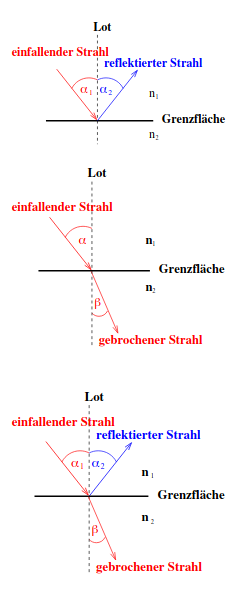
\includegraphics[width=0.35\textwidth]{dreidinger.png}
    \caption{Reflexion und Beugung eines Lichtstrahls. (Quelle \cite{versuch})}
    \label{fig:schemata}
\end{figure}

\subsubsection{Planparallele Platten}
Besitzt ein Körper parallele Grenzflächen, so werden an beiden Grenzflächen
die ankommenden Lichtstrahlen nach den oben genannten Gesetzen aufgeteilt.
Ein Teil des Lichts wird also zwei mal gebrochen und tritt aus der anderen Seite
des Körpers wieder hinaus. Seine Richtung verändert sich allerdings nicht,
da sich beim zweiten Übergang die Brechungsindizes vertauschen, heben sich die
Brechungen gegenseitig auf.
\begin{align*}
    \text{sin}\alpha_1 = n \text{sin}\beta \\
    \text{sin}\beta = \frac{1}{n} \text{sin}\alpha_2\\
    \implies \text{sin}\alpha_1 = \text{sin}\alpha_2
\end{align*}
Allerdings verläuft der Lichtstrahl dennoch nicht gradlinig durch den Körper,
er tritt versetzt aus. Es wird auch vom Strahlversatz gesprochen. Dies ist 
in Abbildung \ref{fig:platten} dargestellt.

\begin{figure}
    \centering
    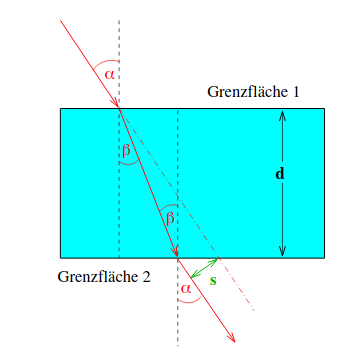
\includegraphics[width=0.35\textwidth]{parallel.png}
    \caption{Brechung an planparallelen Platten. (Quelle \cite{versuch})}
    \label{fig:platten}
\end{figure}

\subsubsection{Prismen}
Anderes lässt sich beim Betrachten von Prismen beobachten. Hier sind die 
Grenzflächen nicht parallel, sondern treffen sich mit einem Winkel $\gamma$.\\
Insgesamt ändert sich die Ausbreitungsrichtung
durch die zweimalige Brechung um den Winkel
\begin{equation}
    \delta = \left( \alpha_1 + \alpha_2 \right) - \left( \beta_1 - \beta_2 \right)
    \label{eqn:prisma}
\end{equation}
Dabei gelten für die Brechungswinkel $\beta_{1, 2}$ das Brechungsgesetz und $\beta_1 + \beta_2 = \gamma$.
(Siehe Abbildung \ref{fig:prisma} )\\
Auch für die Dispersion ist das Prisma ein übliches Beispiel. Da der Brechungsindex
von der Ausbreitungsgeschwindigkeit des Lichts abhängt, hängt er unweigerlich auch
von der Wellenlänge ab. Bei den planparallelen Platten kommt dieser Effekt 
aufgrund der entgegengesetzten Brechung nicht zum Ausdruck, 
da die Brechung beim Prisma allerdings zwei Male in die selbe Richtung 
erfolgt, ist eine unterschiedliche Dispersion zu erwarten.

\begin{figure}
    \centering
    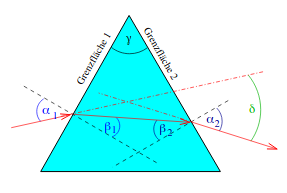
\includegraphics[width=0.35\textwidth]{prisma.png}
    \caption{Brechung am Prisma. (Quelle \cite{versuch})}
    \label{fig:prisma}
\end{figure}

\subsection{Beugung}
Um die sogenannte Beugung zu erklären, die Ausbreitung von Licht im 
Schatten eines Hindernisses, muss der Wellencharakter des Lichts in 
Betracht gezogen werden.\\
Dabei sind die wichtigsten Größen die Frequenz $\nu$, Wellenlänge $\lambda$
und Ausbreitungsgeschwindigkeit $v$. Da Wellen dem Superpositionsprinzip
gehorchen, addieren sich ihre Amplituden und Intensitäten bei Überlagerung.
\\
Haben Wellen dieselbe Frequenz und eine unveränderliche Phasenbeziehung,
so kommt es zur Interferenz. Destruktive Interferenz liegt vor, wenn die 
resultierende Welle abgeschwächt ist, konstruktive Interferenz bei einer
Verstärkung. \\
Ein weiteres wichtiges Prinzip ist das Huygenssche Prinzip, das besagt, dass
an jedem Punkt einer Welle eine Elementarwelle gleicher Frequenz ihren Ausgangspunkt
hat. Diese Wellen werden als Sekundärwellen bezeichnet. Ihre Einhüllende
zeigt die spätere Position der Wellenfront.(vgl. Quelle \cite{versuch})
\\
Das Phänomen der Beugung lässt sich beispielsweise an einem Spalt beobachten.
Beim Auftreffen der ebenen Wellenfront auf den Spalt behalten die gebeugten
Wellen sowohl ihre Frequenz als auch eine feste Phasenbeziehung, sodass auf einem
Detektorschirm ein Interferenzmuster entsteht.\\
Mit der Breite des Spaltes $a$ und der Wellenlänge $\lambda$ gilt für das 
k-te Intensitätsmaximum 
\begin{equation}
    a \text{sin} \alpha = k \lambda
    \label{eqn:einzelspalt}
\end{equation}
$\alpha$ ist dabei der Winkel zur senkrechten Ausbreitungsrichtung.

\subsubsection{Beugung am Gitter}
Für ein Strichgitter, das aus vielen Einzelspalten besteht, ist die Gitterkonstante $d$
der charakterisierende Faktor. Sie besagt, wie viele Spalten pro Längeneinheit 
vorliegen. \eqref{eqn:einzelspalt} wird damit zu
\begin{equation}
    d \text{sin} \alpha = k \lambda
    \label{eqn:strichgitter}
\end{equation}